% !Tex program = pdflatex

\documentclass[UTF8]{ctexart}
\CTEXsetup[format={\Large\bfseries}]{section}
\usepackage{amsmath,amssymb}
\usepackage{hyperref}
\usepackage{parskip}
\usepackage{ctex}
\usepackage{array}
\usepackage{ulem}
\usepackage{graphicx}
\usepackage{booktabs}
\usepackage{listings}
\usepackage{caption}
\usepackage{xcolor}
\usepackage{geometry}
\usepackage{multirow}
\usepackage{subfig}
\usepackage{float}
\usepackage{multicol}
\usepackage{multirow}
\usepackage{pgfplots}
\usepackage{diagbox}
\usepackage{indentfirst}
\setlength {\parindent} {2em} 
% small vertical space between paragraphs for readability
\setlength{\parskip}{0.6em}
\usepackage{makecell}
\geometry{papersize={21cm,29.7cm}}
\geometry{left=2.54cm,right=2.54cm,top=3.18cm,bottom=3.18cm}
\usepackage{fancyhdr}
\pagestyle{fancy}
\DeclareCaptionLabelFormat{figlabel}{#1#2}
\captionsetup[figure]{labelformat=figlabel,name=fig,labelsep=colon}
\lhead{December 1, 2025}
\chead{}
\rhead{2023012274}
\lfoot{Tsinghua University}
\cfoot{\thepage}
\rfoot{Embodied Artificial Intelligence}
\renewcommand{\headrulewidth}{0.4pt}
\renewcommand{\headwidth}{\textwidth}
\renewcommand{\footrulewidth}{0pt}
\usepackage{bm}
% listings style for code snippets
\lstset{
    backgroundcolor=\color{white},
    basicstyle=\ttfamily\small,
    breaklines=true,
    framesep=4pt,
    frame=single,
    rulecolor=\color{gray!40},
    keywordstyle=\color{blue},
    commentstyle=\color{gray!60}\itshape,
    showstringspaces=false,
}
\usepackage{fontspec}
\setmainfont{Georgia}[Mapping=tex-text]
\setsansfont{Georgia}
\setmonofont{Consolas}
\setCJKmainfont{SimSun}

\begin{document}
\begin{titlepage}
     \begin{center}
        \quad \\
        \quad \\
        \quad \\
        \quad \\
        \quad \\
        \quad \\
        \quad \\
        \quad \\ 
        \quad \\ 
        {\kaishu \fontsize{30}{15}\selectfont Embodied Artificial Intelligence}\\
        \quad \\
        \quad \\
        {\kaishu \fontsize{30}{15}\selectfont HW2: Robotics Simulation Workflow}\\

        \end{center}
        \vskip 8cm

        \begin{center}
        \begin{large}
        \begin{tabular}{cc}
        Department:& ~~~~~~~~Department of Automation~~~~~~~~      \\
        \cline{2-2}\\
        Class:& ~~~~~~~~Class 31~~~~~~~~      \\
        \cline{2-2}\\
        Name:& Zuo Gou    \\
        \cline{2-2}\\
        ID:&2023012274   \\
        \cline{2-2}
          \end{tabular}
        \end{large}
      \end{center}

\end{titlepage}
\newpage

\section{Part 1: Hello World}

\subsection{Reproduction}
To reproduce the scene and generate the video, run the following command:
\begin{lstlisting}[language=bash,xleftmargin=2em]
uv run part1/hello_world.py
\end{lstlisting}

\subsection{Scene Construction}
In this part, I constructed a basic Genesis scene using the Genesis framework. The scene consists of a table, four different robots, two object models, and a moving camera.

	\textbf{Table Construction:} The table is built using five boxes: one tabletop and four legs. The tabletop is placed at the center $(0, 0, 0.825)$ with size $(1, 1, 0.05)$, and each leg is positioned at the corners, calculated based on the tabletop and leg sizes. All table components are fixed in the scene.

	\textbf{Robots:}
\begin{itemize}
    \item \textbf{Go2 (Quadruped):} Loaded from its URDF, placed at $(0, -1, 0.42)$, facing the table center (rotated $90^\circ$ about the z-axis). The default joint positions are saved for resetting.
    \item \textbf{G1 (Humanoid):} Loaded from its URDF, placed at $(-0.7, 0, 0.85)$, facing the table center (no rotation needed). Default joint positions are saved.
    \item \textbf{Aloha (Mobile Manipulator):} Loaded from its URDF, placed at $(0, 1, 0.1)$, facing the table center (rotated $-90^\circ$ about the z-axis). Default joint positions are saved.
    \item \textbf{Franka (Robotic Arm):} Loaded from its URDF, placed at $(-0.2, 0, 0.85)$ on the table edge, facing the table center. This arm is fixed in the scene. Default joint positions are saved.
\end{itemize}

	\textbf{Objects:}
\begin{itemize}
    \item \textbf{Airplane:} A mesh model loaded from \texttt{assets/models/Airplane/airplane.obj}, scaled to $0.003$, placed above the table at $(0.2, -0.2, 0.9)$, facing the $+x$ direction (rotated $90^\circ$ about $x$ and $z$).
    \item \textbf{Duck:} A mesh model loaded from \texttt{assets/models/duck/duck.obj}, scaled to $0.0003$, placed at $(0.2, 0.2, 0.9)$, also facing the $+x$ direction.
\end{itemize}

	\textbf{Camera:} A camera is added with resolution $960\times720$, field of view $60^\circ$, near plane $0.1$, and far plane $10.0$. During simulation, the camera orbits the scene in a circular path of radius $2$ at height $2.8$, always looking at the table center $(0, 0, 0.5)$. The camera records a video as it moves.

	\textbf{Robot Control:} If the robots are fixed, their joint positions are reset to the default pose at each step using \texttt{control\_dofs\_position}. This keeps them static for visualization.

\subsection{Results \& Analysis}

The constructed scene visually demonstrates a typical tabletop manipulation setup in simulation. The table is at the center, with four robots (Go2, G1, Aloha, Franka) placed around it, each facing the center for potential interaction. The airplane and duck models are placed on the tabletop as objects to manipulate or observe. The camera orbits the scene, providing a dynamic and comprehensive view of all elements.

\begin{figure}[H]
    \centering
    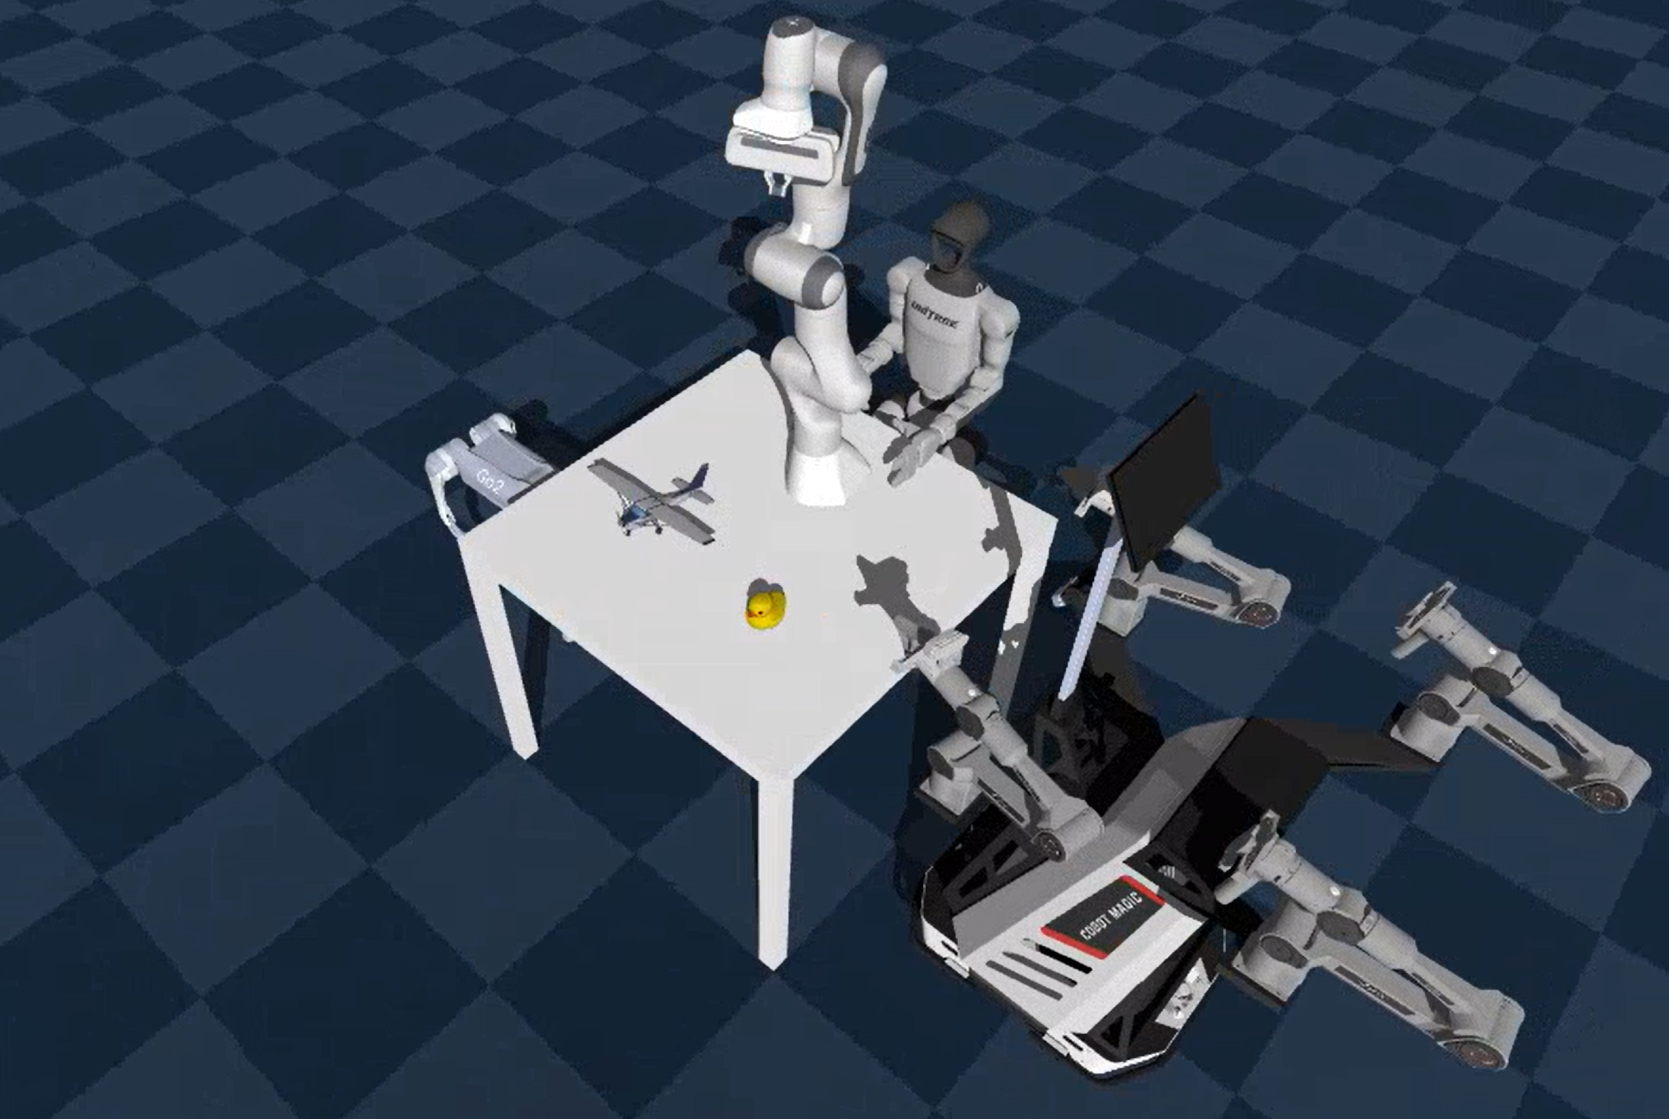
\includegraphics[width=0.8\textwidth]{../part1/hello_world.png} % Replace with actual screenshot
    \caption{Hello World Scene: Table, Robots, and Objects}
    \label{fig:hello_world}
\end{figure}

The output video, \texttt{part1/hello\_world.mp4}, shows the camera smoothly circling the scene, highlighting the spatial arrangement and orientation of all robots and objects. This setup provides a foundation for more complex simulation tasks in later assignments.

\section{Part 2: Sensors}

\subsection{IMU Sensor (Part 2.1)}
\subsubsection{Reproduction}
To run the IMU simulation and generate the acceleration plot:
\begin{lstlisting}[language=bash,xleftmargin=2em]
uv run part2/imu.py
\end{lstlisting}

\subsubsection{Implementation}
In this experiment, I attached a simulated IMU sensor to the end-effector link (\texttt{panda\_link7}) of a Franka Emika Panda robot. The sensor was configured with realistic noise parameters, including acceleration axis skew, bias, and Gaussian noise, to mimic real-world sensor characteristics.

To generate dynamic acceleration data, I implemented a kinematic controller that moves the end-effector along a circular path of radius $0.15$ m centered at $(0.4, 0.0, 0.5)$. The robot's joint positions were computed using inverse kinematics at each time step. During the simulation, I recorded both the raw acceleration readings from the IMU and the ground-truth acceleration provided by the physics engine.

\subsubsection{Analysis}
The IMU sensor was attached to the Franka arm's end-effector. As shown in Figure \ref{fig:imu_plot}, the raw IMU measurements (blue) exhibit significant noise compared to the ground truth acceleration (orange). This demonstrates the importance of filtering or sensor fusion in real-world robotics applications.

% Compare noisy measurements with ground truth.
\begin{figure}[H]
    \centering
    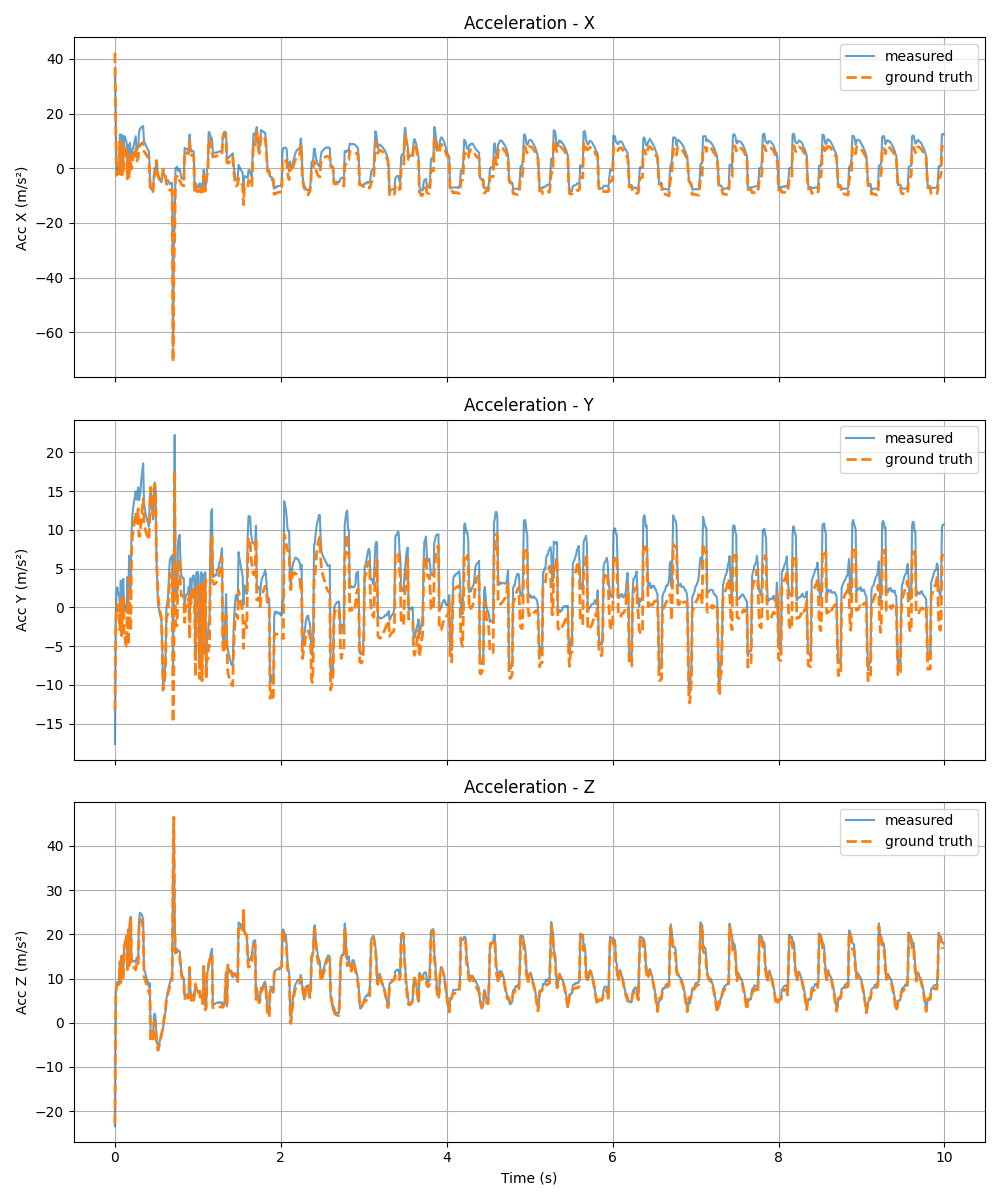
\includegraphics[width=0.6\textwidth]{../part2/imu_acceleration_plot.png}
    \caption{IMU Acceleration Plot: Noisy vs Ground Truth}
    \label{fig:imu_plot}
\end{figure}

\subsection{LiDAR Sensor (Part 2.2)}
\subsubsection{Reproduction}
To simulate the maze navigation and record sensor data:
\begin{lstlisting}[language=bash,xleftmargin=2em]
uv run part2/lidar.py
\end{lstlisting}

To visualize the recorded depth and LiDAR data:
\begin{lstlisting}[language=bash,xleftmargin=2em]
uv run scripts/depth_viz.py --data_path part2/depth_maze_data.npz
uv run scripts/lidar_viz.py --data_path part2/lidar_maze_data.npz
\end{lstlisting}

\subsubsection{Implementation}
I constructed a static maze environment using box primitives based on a $5 \times 5$ grid layout. A Breadth-First Search (BFS) algorithm was implemented to find the shortest path from the start position 'S' to the goal 'G'.

A Unitree Go2 robot was spawned at the start location. I attached two perception sensors to its base link:
\begin{itemize}
    \item \textbf{LiDAR}: A spherical scanning LiDAR with a $360^\circ$ horizontal FOV and $30^\circ$ vertical FOV, configured to sample $512 \times 16$ points per scan.
    \item \textbf{Depth Camera}: A camera sensor outputting depth maps with a resolution of $160 \times 120$ and a horizontal FOV of $60^\circ$.
\end{itemize}

The robot autonomously navigates the calculated path using a simple waypoint tracking controller, which adjusts the robot's yaw rate to face the next waypoint while maintaining a constant forward velocity. Sensor data is recorded at every simulation step for post-processing.

\subsubsection{Visualization \& Analysis}
The robot navigates through the maze while capturing environmental data.
\begin{itemize}
    \item \textbf{Depth Camera}: Captures the distance to obstacles pixel-by-pixel. The visualization shows clear outlines of the maze walls.
    \item \textbf{LiDAR}: Provides a 360-degree point cloud. The visualization demonstrates how the robot perceives the geometry of the maze in real-time.
\end{itemize}

The recorded sensor data is saved in \texttt{part2/depth\_maze\_data.npz} and \texttt{part2/lidar\_maze\_data.npz}.
The visualization videos are \texttt{part2/depth\_viz.mp4} and \texttt{part2/lidar\_viz.mp4}.

\section{Part 3: Tasks}

\subsection{Go2 Locomotion Training}
\subsubsection{Reproduction}
To train the policy:
\begin{lstlisting}[language=bash,xleftmargin=2em]
uv run part3/go2_train.py --max_iterations 1001
\end{lstlisting}

\subsubsection{Environment \& Training}
The training environment is defined in \texttt{part3/go2\_env.py}, inheriting from the Genesis simulation framework. The robot is a Unitree Go2 quadruped with 12 degrees of freedom.

\textbf{Observation Space:} The observation vector (dim=45) includes:
\begin{itemize}
    \item Base linear velocity (3)
    \item Base angular velocity (3)
    \item Projected gravity vector (3)
    \item Joint positions (12) and velocities (12)
    \item Previous actions (12)
\end{itemize}

\textbf{Action Space:} The policy outputs 12 joint position targets, which are processed through a PD controller ($K_p=20.0, K_d=0.5$) with an action scale of 0.25.

\textbf{Reward Design:} The reward function encourages tracking the user-provided velocity commands while maintaining stability and energy efficiency. Key components include:
\begin{itemize}
    \item \textbf{Tracking Rewards:} \texttt{tracking\_lin\_vel} (1.0) and \texttt{tracking\_ang\_vel} (0.2) penalize deviations from the target command $c=(v_x^c, v_y^c, \omega^c)$.
    \item \textbf{Stability Penalties:} \texttt{lin\_vel\_z} (-1.0) penalizes vertical body movement, and \texttt{base\_height} (-50.0) keeps the base near 0.3m.
    \item \textbf{Regularization:} \texttt{action\_rate} (-0.005) and \texttt{similar\_to\_default} (-0.1) encourage smooth motions and natural posture.
\end{itemize}

\textbf{Training:} The policy was trained using PPO (Proximal Policy Optimization) with an Actor-Critic network (hidden layers: [512, 256, 128]) for 1001 iterations.

\subsection{Evaluation}
\subsubsection{Reproduction}
To evaluate the trained policy and generate plots/videos:
\begin{lstlisting}[language=bash,xleftmargin=2em]
uv run part3/go2_eval.py --ckpt 1000
\end{lstlisting}

\subsubsection{Command Tracking Analysis}
I evaluated the trained policy with three commands:
\begin{itemize}
    \item $c_1=(1, 0, 0)$
    \item $c_2=(0, 0.5, 0)$
    \item $c_3=(0, 0, 1)$
\end{itemize}

As shown in Figure \ref{fig:eval_plots}, the robot successfully tracks the commanded velocities.
\begin{itemize}
    \item For $c_1$, the forward velocity $v_x$ converges to 1.0 m/s.
    \item For $c_2$, the lateral velocity $v_y$ tracks 0.5 m/s.
    \item For $c_3$, the yaw rate $\omega$ follows the command of 1.0 rad/s.
\end{itemize}

\begin{figure}[H]
    \centering
    \subfloat[Command $c_1$]{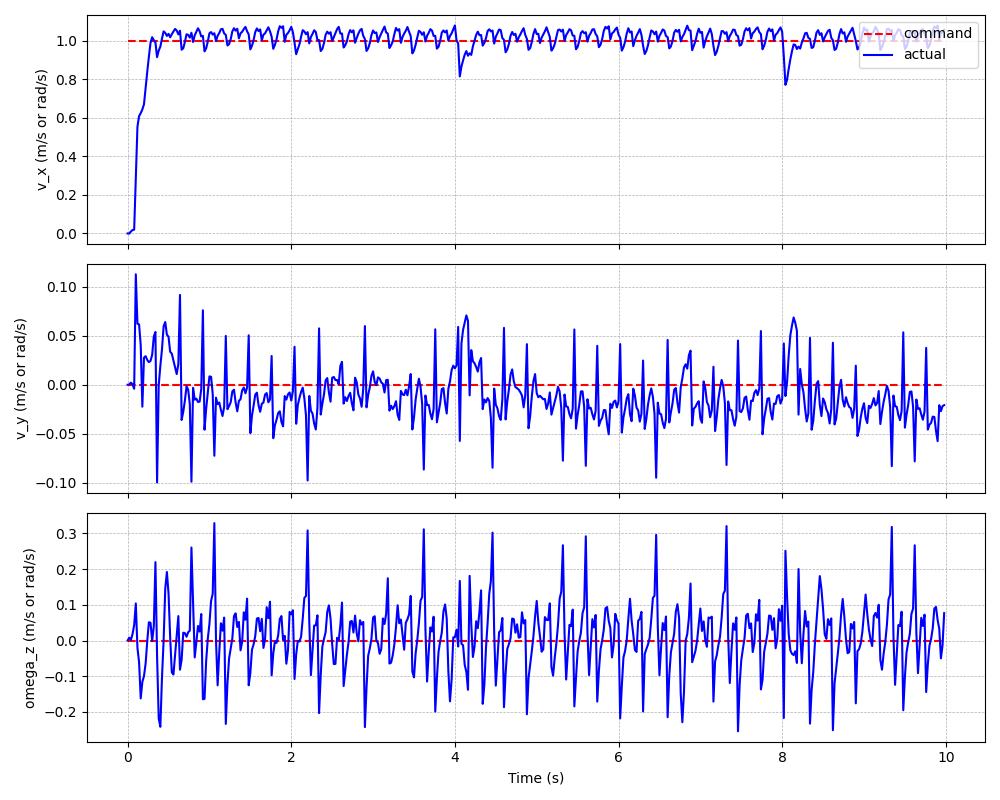
\includegraphics[width=0.32\textwidth]{../part3/eval_c1_plot.png}} \hfill
    \subfloat[Command $c_2$]{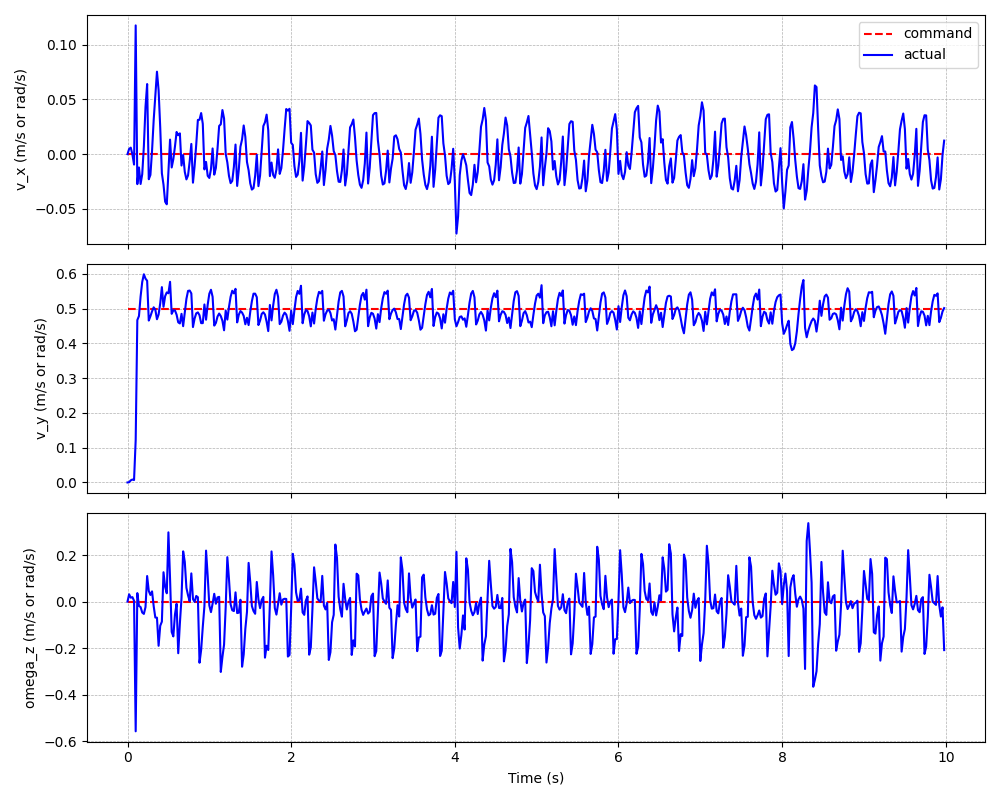
\includegraphics[width=0.32\textwidth]{../part3/eval_c2_plot.png}} \hfill
    \subfloat[Command $c_3$]{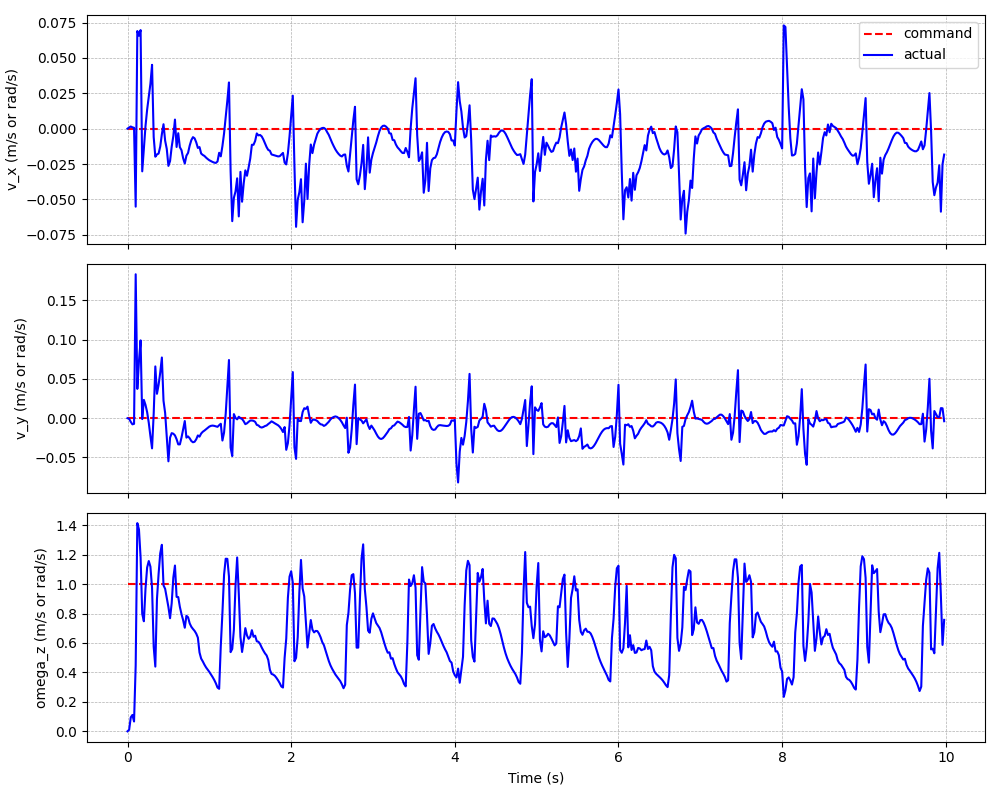
\includegraphics[width=0.32\textwidth]{../part3/eval_c3_plot.png}}
    \caption{Commanded vs Actual Velocities}
    \label{fig:eval_plots}
\end{figure}

The top-down videos for each command are provided in the \texttt{part3} folder.

\subsection{Maze Navigation}
\subsubsection{Reproduction}
To run the maze navigation demo:
\begin{lstlisting}[language=bash,xleftmargin=2em]
uv run part3/go2_maze_run.py --ckpt 1000
\end{lstlisting}

\subsubsection{Implementation}
\textbf{Maze Environment:} The \texttt{Go2MazeEnv} class extends the standard training environment by procedurally generating a maze terrain. The maze layout is defined by a grid string, where walls are constructed using static box primitives. The start 'S' and goal 'G' positions are parsed from the grid to define the navigation task.

\textbf{Navigation Logic:}
The navigation task is solved using a hierarchical approach:
\begin{enumerate}
    \item \textbf{Global Planner:} A Breadth-First Search (BFS) algorithm computes the shortest path of grid cells from the start to the goal. The centers of these cells serve as waypoints.
    \item \textbf{Local Controller:} A pure pursuit-style controller calculates the velocity command $(v_x, v_y, \omega)$ needed to reach the next waypoint.
    \begin{equation}
        v_{cmd} = K_{lin} \cdot R_{yaw}^T \cdot (p_{target} - p_{current})
    \end{equation}
    where $R_{yaw}$ is the robot's heading rotation matrix. The computed commands are fed into the trained locomotion policy to drive the robot.
\end{enumerate}
\subsubsection{Results \& Analysis}
The robot successfully navigated from S to G using the trained locomotion policy. The navigation logic (e.g., waypoint tracking) effectively guided the robot through the corridors. The attached sensors (LiDAR and Depth Camera) provided continuous environmental perception during the run.

\begin{itemize}
    \item Top-down video: \texttt{part3/maze\_topdown.mp4}
    \item Depth visualization: \texttt{part3/maze\_depth\_vis.mp4}
    \item LiDAR visualization: \texttt{part3/maze\_lidar\_vis.mp4}
\end{itemize}

\end{document}
